\documentclass[11pt, conference, letterpaper]{IEEEtran}
\usepackage[utf8]{inputenc} % set input encoding (not needed with XeLaTeX)
%\usepackage{geometry}
%\geometry{letterpaper}
%%% Examples of Article customizations
% These packages are optional, depending whether you want the features they provide.
% See the LaTeX Companion or other references for full information.



\usepackage{graphicx} % support the \includegraphics command and options

% \usepackage[parfill]{parskip} % Activate to begin paragraphs with an empty line rather than an indent

%%% PACKAGES
\usepackage{url}
\usepackage{booktabs} % for much better looking tables
\usepackage{array} % for better arrays (eg matrices) in maths
\usepackage{paralist} % very flexible & customisable lists (eg. enumerate/itemize, etc.)
\usepackage{verbatim} % adds environment for commenting out blocks of text & for better verbatim

\usepackage{subcaption}
%\usepackage{subfig} % make it possible to include more than one captioned figure/table in a single float
\usepackage{algorithm} 
\usepackage{algorithmic}
\usepackage{amsmath}
\usepackage[font=small]{caption}
\usepackage{afterpage}



% These packages are all incorporated in the memoir class to one degree or another...

%%% HEADERS & FOOTERS
%\usepackage{fancyhdr} % This should be set AFTER setting up the page geometry
%\pagestyle{fancy} % options: empty , plain , fancy
%\renewcommand{\headrulewidth}{0pt} % customise the layout...
%\lhead{}\chead{}\rhead{}
%\lfoot{}\cfoot{\thepage}\rfoot{}

%%% END Article customizations

%%% The "real" document content comes below...

\title{A Distributed Greedy Heuristic for Computing Voronoi Tessellations With Applications Towards Peer-to-Peer Networks}
%\author{Double Blind}
\author{Brendan Benshoof \qquad Andrew Rosen \qquad Anu G. Bourgeois \qquad Robert W. Harrison \\Department of Computer Science, Georgia State University\\  bbenshoof@cs.gsu.edu \qquad rosen@cs.gsu.edu \qquad anu@cs.gsu.edu \qquad rharrison@cs.gsu.edu}
\date{} % Activate to display a given date or no date (if empty),
         % otherwise the current date is printed 

\begin{document}
\maketitle

\begin{abstract}
Computing Voronoi tessellations in an arbitrary number of dimensions is a computationally difficult task.
This problem becomes exacerbated in distributed environments, such as Peer-to-Peer networks and Wireless networks, where Voronoi tessellations have useful applications.

We present our Distributed Greedy Voronoi Heuristic, which approximates Voronoi tessellations in distributed environments.
Our heuristic is fast, scalable, works in any geometric space with a distance and midpoint function, and has interesting applications in embedding metrics such as latency in the links of a distributed network.
\end{abstract}
%  We could use a different config 
% networks are only hpped
% we can do non-euclidean metrics if we have a non-euclidean distance and midpoint definition


\section{Introduction}
\label{sec:intro}

Voronoi diagrams \cite{voronoi} have been used in distributed and  peer-to-peer (P2P) applications for some time. 
They have a wide variety of applications.
Voronoi diagrams can be used as part of distributed hash tables\cite{virtvoro}.
They can be used in coverage detection for wireless networks \cite{carbunar2004distributed}.
Massively Multiplayer Online games (MMOs) can use them to distribute game states and events between players at a large scale \cite{hu2004scalable} \cite{hu2008voronoi} \cite{Backhaus:2007:VAS:1326257.1326266}.

Computing the Voronoi tessellation along with its coprime problem, Delaunay Triangulation, is a well analyzed problem.
There are many algorithms to efficiently compute a Voronoi tessellation given all the points on a plane, such as Fortune's sweep line algorithm \cite{fortune1987sweepline}.
However, many network applications are distributed and many of the algorithms to compute Voronoi tessellations are unsuited to a distributed environment.

In addition, trouble occurs when points are located in spaces with more than two dimensions.
Computing the Voronoi tessellation of $n$ points in a space with $d$ dimensions takes $O(n^{\frac{2d-1}{d}})$ time \cite{watson1981computing}.
Distributed computations often have to resort to costly Monte-Carlo calculations \cite{raynet} in order to handle more than two dimensions.

%We take advantage of the fact that distributed applications are fault-tolerant to accommodate changes in network topology.
%This is especially true for P2P environments.
Rather than exactly solving the Voronoi tessellation, we instead a fast and accurate heuristic to approximate each of the regions of a Voronoi tessellation
This enables fast and efficient formation of P2P networks.
A P2P network built using this heuristic would be able to take advantage of it's available fault-tolerant architecture to route along any inaccuracies that arise.
Our paper presents the following contributions:
\begin{itemize}
	\item We present our Distributed Greedy Voronoi Heuristic (DGVH). 
	The DGVH is a fast, distributed, and highly accurate method whereby nodes calculate their individual regions described by a Voronoi tessellation using the positions of nearby nodes.
	DGVH can work in an arbitrary number of dimensions and can handle non-euclidean distance metrics.
    Our heuristic can also handle toroidal spaces.
	In addition, DGVH can accommodate the calculation of nodes moving their positions and adjust their region accordingly, while maintaining a high degree of accuracy (Section \ref{sec:dgvh}).
    Even where small inaccuracies exist, DVGH will create a fully connected graph.
	\item We discuss what P2P and distributed applications can use DGVH and how  (Section \ref{sec:applications}).
	In particular, we show how we can use DGVH to build a distributed hash table with embedded minimal latency.
	\item We present simulations demonstrating DGVH's efficacy in quickly converging to the correct Voronoi tessellation.
    We simulated our heuristic in networks ranging between size 500 to 10000.
	Our simulations show that a distributed network built DGVH accurately determines the region a randomly chosen point falls in 90\% of the time within 20 cycles and converges near 100\% accuracy by cycle 30.
	\item We present the previous work we have built upon to create our heuristic and what improvements we made with DGVH.
	
\end{itemize}


\section{Distributed Greedy Voronoi Heuristic}
\label{sec:dgvh}


A Voronoi diagram is the partition of a space into cells or regions along a set of objects $O$ such that all the points in a particular region are closer to one object than any other object.  
We refer to the region owned by an object as that object's Voronoi region.
%This cleanly maps to the concept of ownership in DHTs, where nodes are responsible for n
%The Delaunay Triangulation of this same space along the same set of objects is defined by the edges such that no object is inside the circumcircle of any triangle formed by the edges \cite{geoalg}.  
The Voronoi diagram and Delaunay Triangulation are dual problems, as an edge between two objects in a Delaunay Triangulation exists if and only if those object's Voronoi regions border each other.  
This means that solving either problem will yield the solution to both.   
An example Voronoi diagram is shown in Figure \ref{voro-ex}.
For additional information, Aurenhammer \cite{aurenhammer1991voronoi} provides a formal and extremely thorough description of Voronoi tessellation, as well as their applications.


\begin{figure}
	\centering
	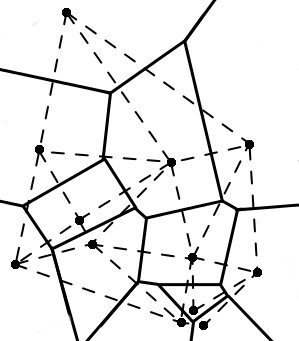
\includegraphics[width=0.75\linewidth]{voronoi}
	\caption{An example Voronoi diagram for objects on a 2-dimensional space.  The black lines correspond to the borders of the Voronoi region, while the dashed lines correspond to the edges of the Delaunay Triangulation.}
	\label{voro-ex}
\end{figure}



\subsection{Our Heuristic}




%take for granted that it requires a fast and efficient way to compute Voronoi tessilations in an arbitrary number of dimensions.
%The Distributed Greedy Voronoi Heuristic (DGVH) is a fast method for nodes to select peers from their Deluanay Triangulation (Algorithm \ref{DGVH}).
The Distributed Greedy Voronoi Heuristic (DGVH) is a fast method for nodes to define their individual Voronoi region (Algorithm \ref{alg:dgvh}). 
This is done by selecting the nearby nodes that would correspond to the points connected to it by a Delaunay triangulation.
The rationale for this heuristic is that, in the majority of cases, the midpoint between to nodes falls on the common boundary of their Voronoi regions.

%In addition, nodes should only have to compute their own Voronoi region, and possibly estimate those of its neighbors. 
%Anything else is a waste of processing power.



\begin{algorithm} % make smaller
\caption{Distributed Greedy Voronoi Heuristic}
\label{alg:dgvh}
\begin{algorithmic}[1]  % the numberis how many lines
	 \STATE Given node $n$ and its list of $candidates$.
   	 \STATE Given the minimum $table\_size$
    \STATE $short\_peers \leftarrow$ empty set that will contain $n$'s one-hop peers
	 \STATE $long\_peers \leftarrow$ empty set that will contain $n$'s two-hop peers    
    \STATE Sort $candidates$ in ascending order by each node's distance to $n$
    \STATE Remove the first member of $candidates$ and add it to $short\_peers$
    \FORALL{$c$ in $candidates$}
    	\STATE $m$ is the midpoint between $n$ and $c$
        \IF{Any node in $short\_peers$ is closer to $m$ than $n$}
        	\STATE Reject $c$ as a peer
        \ELSE
        	\STATE Remove $c$ from $candidates$
        	\STATE Add $c$ to $short\_peers$
        \ENDIF
    \ENDFOR
    \WHILE{$|short\_peers| < table\_size$ \AND $|candidates| >0$}
    	\STATE Remove the first entry $c$ from $candidates$
    	\STATE Add $c$ to $short\_peers$
    \ENDWHILE
    	\STATE Add $candidates$ to the set of $long\_peers$	
    	\IF{$|long\_peers| > table\_size^2$}
        		\STATE $long\_peers \leftarrow$ random subset of $long\_peers$ of size $table\_size^2$
      \ENDIF
\end{algorithmic}
\end{algorithm}


Each cycle, nodes exchange their peer lists with a current neighbor and then recalculate their neighbors.  
A node combines their neighbor's peer list with its own to create a list of candidate neighbors.
This combined list is sorted from closest to furthest.
A new peer list is then created starting with the closest candidate.
The node then examines each of the remaining candidates in the sorted list and calculates the midpoint between the node and the candidate.
If any of the nodes in the new peer list are closer to the midpoint than the candidate, the candidate is set aside.  
Otherwise the candidate is added to the new peer list.







% \subsubsection*{The following paragraphs may need reordering}


DGVH never actually solves for the actual polytopes that describe a node's Voronoi region.
This is unnecessary and prohibitively expensive \cite{raynet}.
Rather, once the heuristic has been run, nodes can determine whether a given point would fall in it's region.

Nodes do this by calculating the distance of the given point to itself and other nodes it knows about.
The point falls into a particular node's Voronoi region if it is the node to which it has the shortest distance.
This process continues recursively until a node determines that itself to be the closest node to the point.
Thus, a node defines its Voronoi region by keeping a list of the peers that bound it.



%maybe move this paragraph to analysis
This heuristic has the benefit of being fast and scalable into any geometric space where a distance function and midpoint can be defined.
The distance metric used for this paper is the minimum distance in a multidimensional unit toroidal space.
Where $\vec{a}$ and $\vec{b}$ are locations in a $d$-dimensional unit toroidal space:
\[ distance = \sqrt{\sum\limits_{i\in d} (\min(|\vec{a}_i-\vec{b}_i|, 1-|\vec{a}_i-\vec{b}_i|))^2}\]
As a result, whether distance and abstract term relating to an overlay or corresponds to physical distance depends on the application.

%In two-dimensional spaces, there is quick hack to achieve 100\% accuracy distributed.

Our heuristic can be overaggressive in removing candidate nodes.
For example, if a node is located between two other nodes, such that their midpoint does not fall upon the shared face of their Voronoi regions, then this heuristic will not link the blocked peers.
This is demonstrated in Figure \ref{occ-ex}.
\begin{figure}
	\centering
	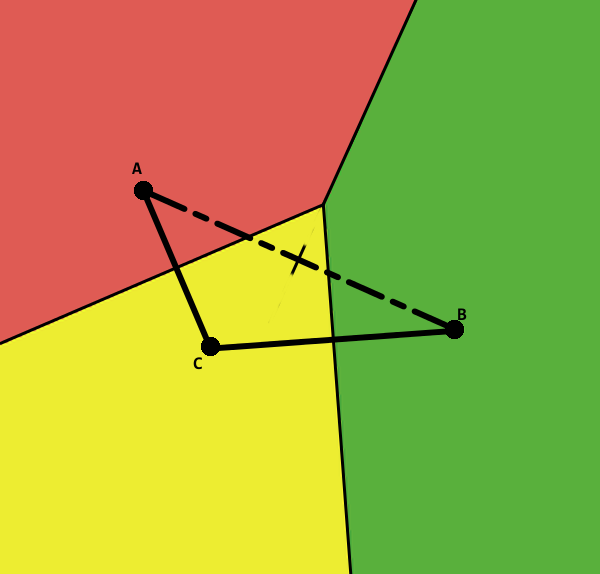
\includegraphics[width=\linewidth]{occlusion}
	\caption{The edge between $A$ and $B$ is not detected by DGVH, as node $C$ is closer to the midpoint than $B$ is.  This is mitigated by peer management polices.}  %Add labels a b c and reference the node labels in text
	\label{occ-ex}
\end{figure}
Our algorithm handles these cases via our method of peer management (Section \ref{sec:manage}).
%Overaggressive pruning by a single nodes is handled by neighboring nodes. 
%So long as a single node determines that an edge exists, it will advertise that edge's existence.









\subsection{Peer Management}
\label{sec:manage}
Nodes running the heuristic maintain two peer lists: \textit{Short Peers} and \textit{Long Peers}.
This is done to  mitigate the error induced by DGVH and providing robustness against churn\footnote{The disruption caused to an overlay network by the continuous joining, leaving, and failing of nodes.} in a distributed system.

\textit{Short Peers} are the set of peers DGVH judged to have Voronoi regions adjacent to the node's own. 
Using a lower bound on the length of \textit{Short Peers} corrects for errors in the approximation as it force nodes to include peers in that would otherwise be omitted. 
Previous work by Beaumont \textit{et al}.\ \cite{raynet} has found a useful lower bound on short peers to be $3d + 1$.
Should the number of short peers generated by DGVH be less than the lower bound, the nearest peers not already included in \textit{Short Peers} are added to it, until \textit{Short Peers} is of sufficient size.
%Members of \textit{Short Peers} are analogous to the predecessors/successors in other DHTs.



There is no upper bound to the number of short peers a node can have.
This means in contrived cases, such as a single node surrounded by other nodes forming a hypersphere, this number can grow quite high.
Bern \textit{et al.\ }\cite{bern1991expected} found that the expected maximum degree of a vertex in a Delaunay Triangulation is
$$\Theta(\frac{\log n}{\log \log n} )$$ 
where $n$ is the number of nodes in the Delaunay Triangulation. 
This bound applies to a Delaunay Triangulation in any number of dimensions.
Thus, the maximum expected size of \textit{Short Peers} is bounded by $\Theta(\frac{\log n}{\log \log n} )$, which is a highly desirable number in many distributed systems \cite{chord} \cite{kademlia}.



\textit{Long Peers} is the list of two-hop neighbors of the node.
When a node learns about potential neighbors, but are not included in the short peer list, they may be included in the long peer list.  
\textit{Long Peers}has a maximum size of $(3d+1)^2$, although this size can be tweaked to the user's needs.  
For example, if \textit{Short Peers} has a minimum size of 8, then \textit{Long Peers} has a maximum of 64 entries.  
We recommend that members of \textit{Long Peers} are not actively probed during maintenance to minimize the cost of maintenance.
A maximum size is necessary, as leaving it unbounded would result in a node eventually keeping track of all the nodes in the network, which would be counter to the design of a distributed and scalable system

%We next discuss how nodes learn about short and long peers.
How nodes learn about peers is up to the application.
We experimented using a gossip protocol, whereby a node selects peer from \textit{Short Peers} at random to ``gossip'' with.
When two nodes gossip with each other, they exchange their \textit{Short Peers} with each other.
The node combines the lists of short peers\footnote{Nodes remove themselves and repetitions from the candidates they receive.} and uses DGVH to determine which of these candidates correspond to its neighbors along the Delaunay Triangulation.
The candidates determined not to be short peers become long peers.  
If resulting number of long peers exceeds the maximum size of \textit{Long Peers}, a random subset of the maximum size is kept.

The formal algorithm for this process is described in Algorithm~\ref{alg:gossip}.
This maintenance through gossip process is very similar to the gossip protocol used in Beaumont et al.'s RayNet \cite{raynet}.


\begin{algorithm}
\caption{Gossiping}
\label{alg:gossip}
\begin{algorithmic}[1]  % the number is how many 
	\STATE Node $n$ initiates the gossip.
	\STATE $neighbor \leftarrow$ random node from $n.short\_peers$
   \STATE $n\_candidates \leftarrow n.short\_peers \cup n.long\_peers \cup neighbor.short\_peers$
   \STATE $neighbor\_candidates \leftarrow neighbor.short\_peers \cup neighbor.long\_peers \cup n.short\_peers$.  
   \STATE $n$ and $neighbor$ each run Distributed Greedy Voronoi Heuristic using their respective $candidates$
\end{algorithmic} 
\end{algorithm}


\subsection{Algorithm Analysis}

DVGH is very efficient in both terms of space and time.
Suppose a node $n$ is creating its short peer list from $k$ candidates in an overlay network of $N$ nodes. 
The candidates must be sorted, which takes $O(k\cdot\lg(k))$ operations.  
Node $n$ must then compute the midpoint between itself and each of the $k$ candidates.  
Node $n$ then compares distances to the midpoints between itself and all the candidates.  
This results in a cost of 

\[ k\cdot\lg(k) + k \text{ midpoints}  + k^{2} \text{ distances} \]


Since $k$ is  bounded by $\Theta(\frac{\log N}{\log \log N} )$ \cite{bern1991expected} (the expected maximum degree of a node?), we can translate the above to

\[O(\frac{\log^{2} N}{\log^{2} \log N} )\]

In the vast majority of cases, the number of peers is equal to the constant minimum table size. 
This yields $k=(3d+1)^2+3d+1$ in the expected case, where the lower bound and expected complexities are $\Omega(1)$.

Previous work \cite{raynet} claims constant time approximation. 
The reality is that Raynet's leading constant is in the order of thousands. % as Monte-Carlo samples.  
Our algorithm has a greater asymptotic worst case cost, but for all current realistic network sizes it will be more time efficient then RayNet's approximation.

\section{Applications}
\label{sec:applications}

As we previeously discussed in Section \ref{sec:intro} Voronoi tessellation has many applications for distributed systems.

We focus our discussion on the two extremes of applications: DHTs, which deal with overlays, and wireless networks, which need to take literal physical constraints into account.

\subsection{Distributed Hash Tables}
Arguably all Distributed Hash Tables (DHTs) are built on the concept of Voronoi tessellation.
In all DHTs, a node is responsible for all points in the overlay to which it is the ``closest'' node.
Nodes are assigned a key as their location in some keyspace, based on the hash of some attributes.
Normally, this is just the hash of the IP address and port of the node  \cite{chord} \cite{kademlia} \cite{can} \cite{pastry}, but other metrics such as geographic location can be used as well \cite{ratnasamy2002ght}.

These DHTs have carefully chosen metric spaces such that these regions are very simple to calculate.
For example, Chord and similar ring-based DHTs utilize a unidirectional, one-dimensional ring as their metric space, such that the region for which a node is responsible is the region between itself and its predecessor.

Using a Voronoi tessellation in a DHT generalizes this design. 
Nodes are Voronoi generators at a position based on their hashed keys.
These nodes are responsible for any key that falls within its generated Voronoi region.

Messages get routed along links to neigboring nodes. 
This would take $O(n)$ in one dimension.
In multiple dimensions, our routing algorithm (Algorithm \ref{alg:lookup}) is extremely similar to the one used in CAN, which is bounded by a runtime of $O(n^{\frac{1}{d}})$.
\begin{algorithm}
	\caption{Lookup in a Voronoi-based DHT}
	\label{alg:lookup}
	\begin{algorithmic}[1] 
		\STATE Given node $n$
		\STATE Given $m$ is a message addressed for $loc$
		\STATE $potential\_dests \leftarrow n \cup n.short\_peers \cup n.long\_peers$ ????
		\STATE $c \leftarrow $ node in $ potential\_dests$ with shortest distance to $loc$
		\IF{$c$ == $n$}
		\RETURN $n$
		\ELSE
		\RETURN $c.lookup(loc)$
		\ENDIF
	\end{algorithmic}
\end{algorithm}

DGVH can be used in a DHT to quickly and scabaly construct both the Voronoi tessilation and links to peers.
%TODO Numbers to back up needed?
In addition, gossip-based peer management policies are extremely efficient in proactively handling node joins and failures.
A join operation should inform nearby nodes immediately.
This can be done by the joiner contacting each peer in the peer lists of the node previously responsible for the joiner's location, 

Node failures can be handled extremely lazily.When a node.
When a node attampts to route to or gossip with a node and discovers it no longer exists, it should remove the node from its peer lists and inform all of the nodes it knows to do the same.
Since routing is how a node would make a decision on whether a point belongs to a particular Voronoi region, failed nodes don't have any impact on the network's accuracy.



Multiple metric spaces



\subsection{Embedding Routing Information in Metric Spaces}


During previous research in applications of DHTs \cite{andrew-poster} to parallel processing, we tested DHT network behavior under churn. 
We came to the conclusion that high levels of churn improved the performance of the system under certain circumstances.
The built-in mechanisms for managing responsibility in a DHT are very effective and efficient at handling nodes changing locations in the network.
In this work we found that it was more effective to move the node to a location in the DHT where work or data was stored rather than attempt to remap data efficiently over the nodes.


Voronoi tesselation can be used to design DHTs which leverage this discover.
A nodes' location in the network can be used to provide meaningful information about the node and to allow nodes to change location in the network to suit the networks needs.
In this paper we propose a method that enables peers to periodically change their location in the network such that routes taken on the resulting overlay network have lower latency than would otherwise possible in a DHT.
Each node is given a random initial location and, over time, migrates to a location which optimizes latency.

A good example of this is embedding latency as a dimension.
Every DHT uses the number of hops as a metric of routing speed, but in reality, the number of hops is an estimation of what is really wanted: a measure of latency.

\subsection{Wireless Coverage}
C\u{a}rbunar et al.\ \cite{carbunar2004distributed} demonstrated how Voronoi tessellation could be used to solve the \textit{coverage-boundary} problem in wireless ad-hoc networks.
The coverage-boundary problem asks which nodes are on the physical edge of the network.
This knowledge provides useful information to networks.
For example, ad-hoc networks operating in with no infrastructure or have been set up temporarily can use this knowledge to define the reach of the network's coverage.


\section{Experiments}
\label{sec:experiments}


We implemented two sets of experiments for DGVH.
The first compares the Voronoi tessellations created by DGVH to actual Voronoi tessellation.
Our second set of experiments demonstrate that DGVH's errors are of little consequence when building a distributed and fault-tolerant systems.


Distance

\subsection{Experiment 1:  Voronoi Accuracy}

\subsection{Experiment 2: P2P Convergence and Routing}
Our second set of experiments examines how DGVH could be used to create a DHT and how well it would perform in this task.
Our simulation demonstrates how DGVH  can be used to create a stable overlay from a chaotic starting topology after a sufficient number of gossip cycles.  
We do this by showing that the rate of successful lookups approaches 1.0.
We compare these results to RayNet \cite{raynet}, which proposed that a random $k$-connected graph would be a good, challenging starting configuration for demonstrating convergence of a DHT to a stable network topology.

During the first two cycles of the simulation, each node bootstraps its short peer list by appending 10 nodes, selected uniformly at random from the entire network.
In each cycle, the nodes gossip (Algorithm \ref{alg:gossip}) and run DGVH using the new information.
We then calculate the hit rate of successful lookups by simulating 2000 lookups from random nodes to random locations, as described in Algorithm \ref{routesim}.
A lookup is successful when the network correctly determines which Voronoi region contains a randomly selected point.


Our experimental variables for this simulation were the number of nodes in VHash overlay and the number of dimensions.  
We tested network sizes of 500, 1000, 2000, 5000, and 10000 nodes each in 2, 3, 4, and 5 dimensions.
The hit rate at each cycle is $\frac{hits}{2000}$, where $hits$ are the number of successful lookups.




\begin{algorithm}
	\caption{Routing Simulation Sample}
	\label{routesim}
	\begin{algorithmic}[1]  % the number is how many 
		\STATE $start \leftarrow$ random node
		\STATE $dest \leftarrow$ random set of coordinates
		\STATE $ans \leftarrow$ node closest to $dest$
		\IF{$ans == start.lookup(dest)$}
		\STATE increment $hits$
		\ENDIF
	\end{algorithmic} 
\end{algorithm}


%In order to show that leaving the size of the short peer list unbounded is not detrimental to the memory costs of nodes, we also kept track of the size of the short peer list at each cycle. 

%\subsection{Convergence Simulation Results}
Our results are shown in Figures \ref{conv2}, \ref{conv3}, \ref{conv4}, and \ref{conv5}.
Our graphs show that the created overlay quickly constructs itself from a random configuration and that our hit rate reached 90\% by cycle 20, regardless of dimension.
Lookups consistently approached a hit rate of 100\% by cycle 30. 
In comparison, RayNet's routing converged to a perfect hit rate at around cycle 30 to 35 \cite{raynet} 
As the network size and number of dimensions each increase, convergence slows, but not to a significant degree.

\begin{figure*}
	\centering 
	\begin{tabular}{cc}
		
		\begin{subfigure}{\columnwidth}
			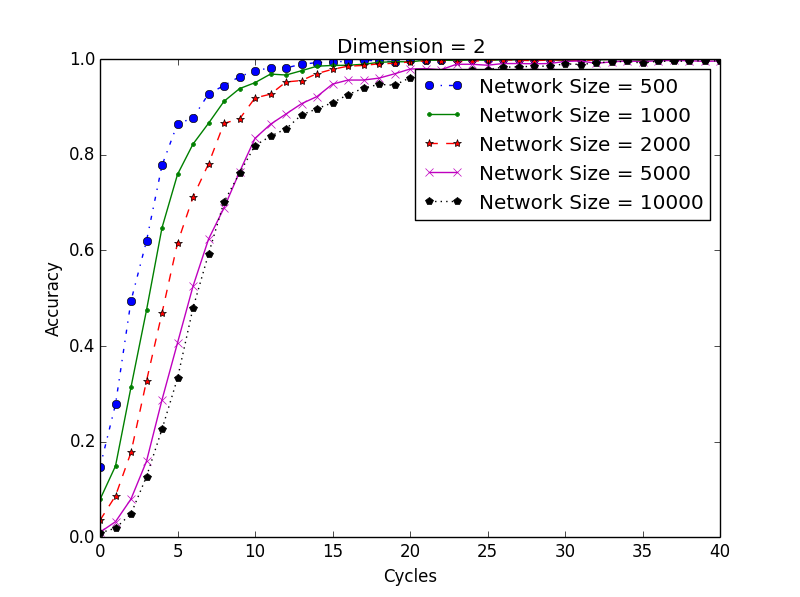
\includegraphics[width=\columnwidth]{conv_d2}
			\caption{This plot shows the accuracy rate of lookups on a 2-dimensional VHash network as it self-organizes.}
			\label{conv2}
		\end{subfigure} &
		
		\begin{subfigure}{\columnwidth}
			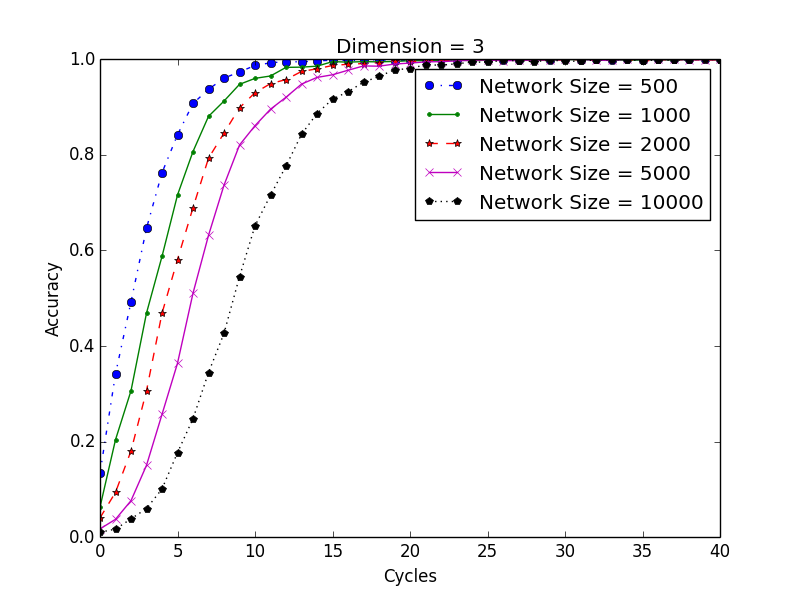
\includegraphics[width=\columnwidth]{conv_d3}
			\caption{This plot shows the accuracy rate of lookups on a 3-dimensional VHash network as it self-organizes.}
			\label{conv3}
		\end{subfigure} \\
		
		\begin{subfigure}{\columnwidth}
			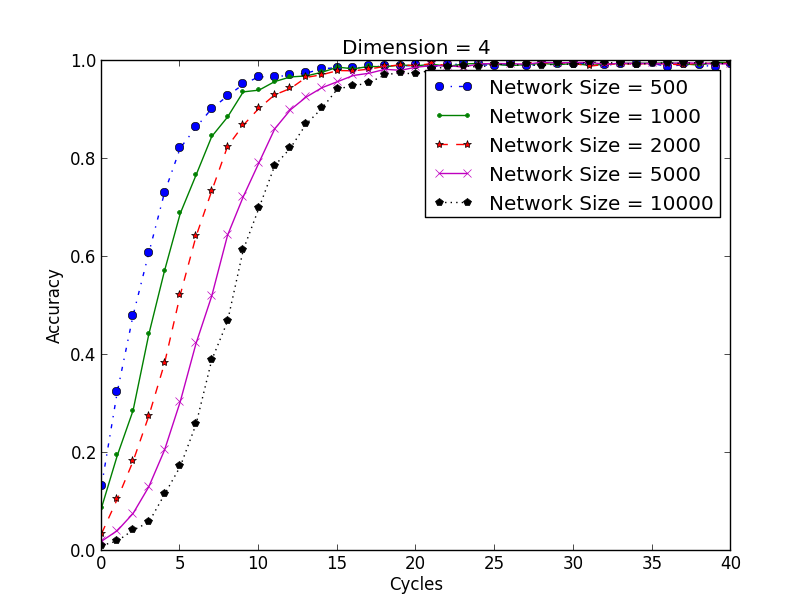
\includegraphics[width=\linewidth]{conv_d4}
			\caption{This plot shows the accuracy rate of lookups on a 4-dimensional VHash network as it self-organizes.}
			\label{conv4}
		\end{subfigure} &
		
		
		\begin{subfigure}{\columnwidth}
			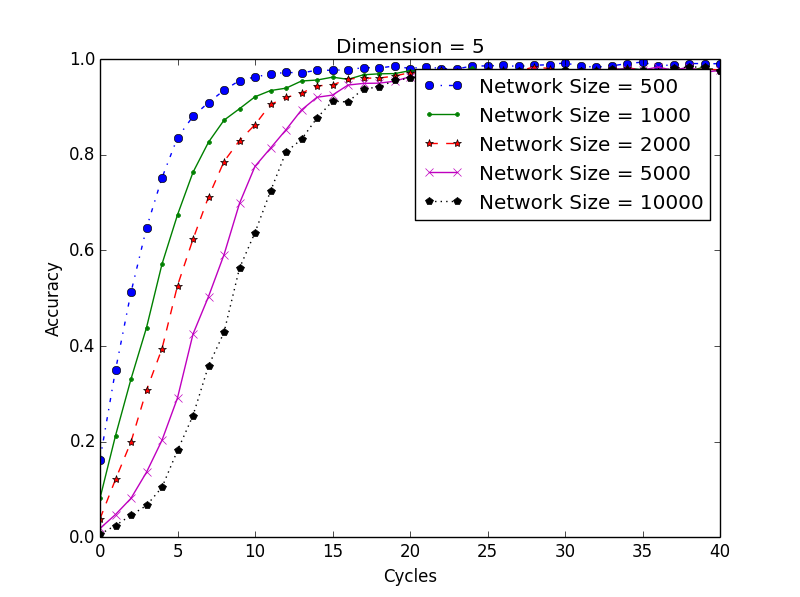
\includegraphics[width=\linewidth]{conv_d5}
			\caption{This plot shows the accuracy rate of lookups on a 5-dimensional VHash network as it self-organizes.}
			\label{conv5}
		\end{subfigure}
		
	\end{tabular}
	
	\caption{These figures show that, starting from a randomized network, VHash forms a stable and consistent network topology.
		The Y axis shows the success rate of lookups and the X axis show the number of gossips that have occurred.
		Each point shows the fraction of 2000 lookups that successfully found the correct destination.}
	
\end{figure*}
%\begin{table}
%\centering
%\begin{tabular}{|r|r|r|r|}
%\hline
%Network Size & Dimensions & avg degree & max degree\\ \hline
%500   & 2 & 7.004 & 8 \\ \hline
%1000  & 2 & 7.001 & 8 \\ \hline
%2000  & 2 & 7.0015 & 8 \\ \hline
%5000  & 2 & 7.0364 & 66 \\ \hline
%10000 & 2 & 8.0151 & 81\\ \hline  % the heck?
%500   & 3 & 10.364 & 16 \\ \hline
%1000  & 3 & 10.321 & 15 \\ \hline
%2000  & 3 & 10.272 & 16 \\ \hline
%5000  & 3 & 10.3264 & 18 \\ \hline
%10000 & 3 & 9.1233 & 19 \\ \hline
%500   & 4 & x & x \\ \hline
%1000  & 4 & x & x \\ \hline
%2000  & 4 & x & x \\ \hline
%5000  & 4 & x & x \\ \hline
%10000 & 4 & x & x \\ \hline
%500   & 5 & x & x \\ \hline
%1000  & 5 & x & x \\ \hline
%2000  & 5 & x & x \\ \hline
%5000  & 5 & x & x \\ \hline
%10000 & 5 & x & x \\ \hline
%\end{tabular}
%\caption{Information about the size short peer lists, denoted degree here, at the last cycle of the convergence simulation.  For each pair of network size and dimension, we report the average degree in the network, as well as the largest.}
%\label{tab:convtable}
%\end{table}


\section{Related Work}
\label{sec:related}
%check table size consistancy 
While there has been previous work on applying Voronoi regions to DHTs and peer-to-peer (P2P) applications, we have found no prior work on how to perform embedding of an inter-node latency graph.   

Backhaus et al.'s  VAST \cite{Backhaus:2007:VAS:1326257.1326266} is a Voronoi-based P2P protocol designed for handling event messages in a massively multiplayer online video game.  
Each node finds its neighbors by constructing a Voronoi diagram using Fortune's sweepline algorithm \cite{fortune1987sweepline}.  
VAST demonstrated that Voronoi diagrams could be used as the backbone to large-scale applications, although their work focused specifically on using 2-dimensional Voronoi diagrams.
VAST could use   
VHash approximates the Voronoi region rather than solving it, as higher dimension Voronoi regions are computationally expensive to solve.

The two DHT protocols developed by Beumont et al., VoroNet \cite{voronet} and RayNet \cite{raynet} are the closest comparisons to VHash.
VoroNet is based off Kleinberg's small world model \cite{kleinberg2000navigation} and achieves polylogarithmic lookup time.  
Each node in Voronet solves its Voronoi region to determine its neighbors and also maintains a link to a randomly chosen distant node.
Voronet focused specifically on the two-dimensional Voronoi computations and the techniques used would be too expensive in higher dimensions and were not resilient to churn  \cite{raynet}.

RayNet \cite{raynet} was based on the work done on Voronet and used a heuristic to calculate Voronoi tessilations.  
Like our DGVH, RayNet's heuristic does not solve for Voronoi regions, as that is prohibitively expensive.  
RayNet uses a Monte-Carlo method to approximate the volume of a node's Voronoi region in constant time.  
While effective at estimating the Voronoi region,  the volume-based Monte-Carlo approximation is expensive and requires multiple samples. 
This gives the runtime of RayNet's heuristic an enormous leading constant.
RayNet does mention the idea of mapping attributes to each axis, but how this can be exploited is left as future work.




%Unlike ACE, we handle unbounded simultaneous join and leave operations.



\section{Conclusion}
\label{sec:conclusion}


We ran two 
Our first experiments demonstrate that our heuristic is ``mostly correct'' and our second set demonsrates that ``mostly correct'' is sufficient to build a P2P network which can route accurately.



Another venue for exploration is application of caching and replication strategies to a functional distributed file system running on top of VHash.  Such extensions seek to improve upon existing work done on file replication and caching schemes \cite{shen2010irm}.





\bibliographystyle{ieeetr}
\bibliography{P3DNS}
\end{document}
